\documentclass[11pt]{article}

\usepackage[utf8]{inputenc}
\usepackage{amsmath,amssymb,color,enumitem,fancyvrb,float,hyperref,graphicx,geometry,listings,mathtools,nicefrac,url}
\usepackage[english]{babel}
\usepackage[tt=false,type1=true]{libertine}
\usepackage[varqu]{zi4}
\usepackage[numbib]{tocbibind}
\usepackage{parskip}

\usepackage{listings}     
\usepackage{lstautogobble}

\lstset{
    autogobble,
    language=python,
    columns=fullflexible,
    showspaces=false,
    showtabs=false,
    breaklines=true,
    showstringspaces=false,
    breakatwhitespace=true,
    escapeinside={(*@}{@*)},
    basicstyle=\ttfamily\footnotesize,
    frame=l,
    framesep=12pt,
    xleftmargin=12pt,
    tabsize=2,
    captionpos=b,
    numbers=left,
    xleftmargin=4em,
    framexleftmargin=1em
}

%\lstnewenvironment{code}[2]{\lstset{caption=#1, label=#2 , keepspaces=true}\minipage{\linewidth}\smallskip}{\medskip\endminipage}
\lstnewenvironment{code}[2]{\lstset{caption=#1, label=#2 , keepspaces=true}\smallskip}{\medskip}

\renewcommand{\footnotesize}{\scriptsize}

\hypersetup{
    colorlinks = true,
    allcolors = {black}
}

\geometry{
 	left=35mm,
 	right=35mm,
}

\title{\vspace*{-3em}\huge \textbf{Investigating Manifold Mixup}\\[0.25em] \large \textit{Computer Vision WS19/20}\\[0.5em]}
\date{}
\author{
	Julian Kanzler \and
	Michael Nening \and
	Manuel Widmoser
}

\begin{document}
\maketitle

\begin{abstract}
	\noindent In this work, we investigate manifold mixup, a simple regularizer that encourages deep neural networks to predict less confidently on adversarial examples. 
    We evaluate manifold mixup on a subset of CIFAR-10, where we only use ten percent of the training examples.
    In our experiments, we first attempt to get the baseline high by considering different preprocessing steps, learning rate schedulers and hyperparameters.
    Then, manifold mixup with different $\alpha$-values, which controls the strength of interpolation between feature-target pairs, is applied.
    We find \dots
\end{abstract}

\section{Introduction}
\label{sec:introduction}

Deep neural networks often give incorrect but still highly confident predictions when evaluated on data which only comes from a slightly different distribution than examples from the training data.
This can already be achieved by marginal perturbations that are imperceptible to the human eye.
Such inputs, also known as \textit{adversarial examples}, may be a serious hazard when machine learning systems are used in security-sensitive applications.

To address this issue, the training data can be extended by similar but different examples.
This method is called \textit{data augmentation} and leads to better generalization~\cite{simard96}.
However, data augmentation depends on the dataset, and thus human knowledge is needed.

Mixup is a simple data-agnostic data augmentation procedure that increases the robustness of neural networks when facing adversarial examples by extending the training distribution~\cite{zhang17}.
Mixup provides convex combinations of example/label-pairs where the network additionally will be trained on.
This regularizes the neural network to favor simple linear behavior in-between training examples.

Basically, mixup constructs virtual training examples $(\tilde{x}, \tilde{y})$ such that
\begin{align}
    \tilde{x} &= \lambda x_i + (1 - \lambda) x_j \\
    \tilde{y} &= \lambda y_i + (1 - \lambda) y_j
\end{align}
where $x_i$, $x_j$ are raw input vectors, $y_i$, $y_j$ are one-hot label encodings and $\lambda \sim \text{Beta}(\alpha, \alpha)$ is the mixing coefficient sampled from the Beta distribution dependent on $\alpha$.
$\alpha = 1.0$ is equivalent to sampling $\lambda \sim U(0,1)$.
\section{Manifold Mixup}
\label{sec:manifoldmixup}

Manifold mixup trains neural networks on linear combinations of hidden representations of training examples~\cite{verma19}.
Hence, it performs mixup in an intermediate layer in which feature spaces are more aligned.
Furthermore, a neural network trained with manifold mixup learns class-representations with fewer directions of variance and yields a smoother decision boundary.

Training a deep neural network using manifold mixup is done as follows:
We select a layer $k$ at random from the set of eligible layers $\mathcal{S}$ in the neural network. 
$\mathcal{S}$ may contain the first layers of the residual blocks, for instance.
Then perform input mixup~\cite{zhang17} on two random minibatches $(x_i, y_i)$ and $(x_j,y_j)$ which are processed through the forward pass until reaching layer $k$. This gives us a mixed minibatch $(\tilde{x}, \tilde{y})$.
With that we continue the forward pass from layer $k$ until we ultimately get the output.
Finally, we update the parameters of the neural network by computing the loss and gradients using the output.

\subsection{Implementation}

Manifold mixup can be implemented in a few lines of code without heavy computations that would drop the training performance of the deep neural network a lot.

\begin{code}{Mixup implementation}{lst:mixup}
def mixup(x, y, alpha):
    batch_size = x.size()[0]
    lam = np.random.beta(alpha, alpha) if mixup_alpha > 0 else 1

    if torch.cuda.is_available():
        index = torch.randperm(batch_size).cuda()
    else:
        index = torch.randperm(batch_size)

    # x[index, :] swaps the training samples
    mixed_x = lam * x + (1 - lam) * x[index, :]
    y_a, y_b = y, y[index]
    
    return mixed_x, y_a, y_b
\end{code}

Listing~\ref{lst:mixup} shows the actual mixup procedure that 
(1) draws $\lambda$ from the Beta distribution (line 3),
(2) picks batch-size many random indices (line 6 and 8, respectively),
(3) mixes each sample in the batch with another sample determined by the random indices (line 11).

\newpage
\subsection{Visualization}

Figure~\ref{fig:visualization} visualizes three examples of the mixup process using $\lambda = 0.5$.

\begin{figure}[ht]
    \centering
    \begin{minipage}{.25\columnwidth}
        \centering
        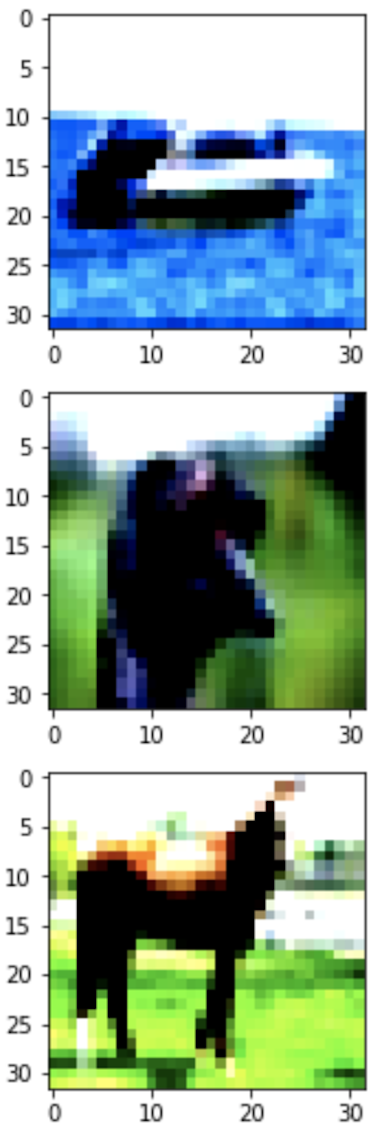
\includegraphics[width=0.7\textwidth]{figures/1.png} \\
        (a)
    \end{minipage}
    \begin{minipage}{.25\columnwidth}
        \centering
        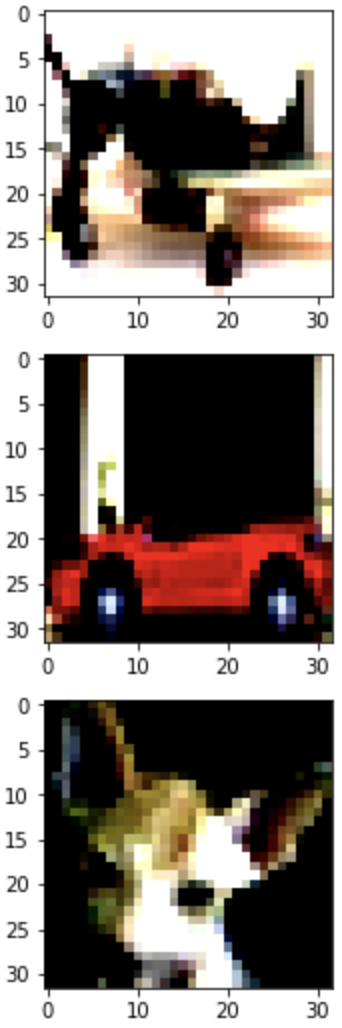
\includegraphics[width=0.7\textwidth]{figures/2.png} \\
        (b)
    \end{minipage}
    \begin{minipage}{.25\columnwidth}
        \centering
        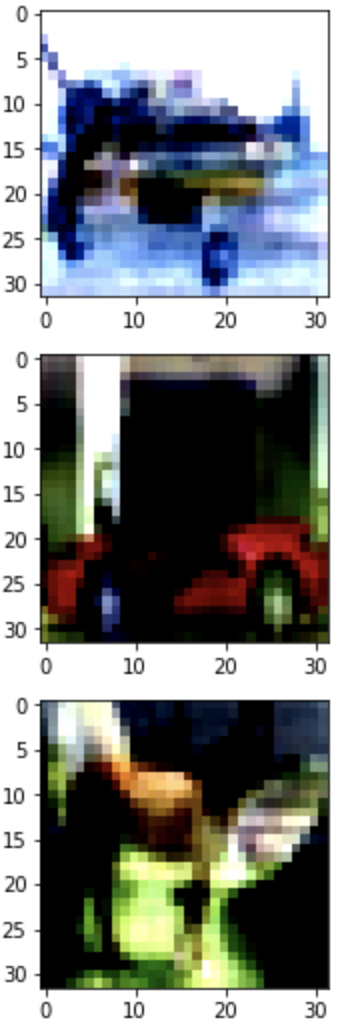
\includegraphics[width=0.7\textwidth]{figures/3.png} \\
        (c)
    \end{minipage}

    \caption{Mixup visualized: (a) and (b) depict two randomly drawn samples, respectively, (c) the mixup outcome of (a) and (b) by setting $\lambda$ to $0.5$. Each row represents a different example.}
    \label{fig:visualization}
\end{figure}
\section{Baseline}
\label{sec:baseline}

All experiments were conducted on a subset of the CIFAR-10 dataset~\cite{krizh09}. This dataset consists of 60.000 images labeled to ten different classes, of which we used only 50 of each class to conduct training. Our intention was to measure the impact of manifold mixup applied to training with such a small set of training examples.

\subsection{Architecture \& Training}

The model used to conduct our experiments consists of three blocks, each implementing three convolution layers (convolution, BatchNorm, LeakyReLU) followed by a pooling and dropout operation. The final layer is a linear layer for classification. Figure~\ref{fig:net} visualizes the full architecture.

\twocolumn

The initial configuration was set to train using stochastic gradient descent (SGD) with the \texttt{StepLR}-scheduler at learning rate of 0.01, weight decay of $1e^{-3}$ and momentum of 0.9. Training was executed for 100 epochs and on batches of 32 images. Random cropping and random horizontal flipping was applied to the training data, as suggested in ~\cite{goyal17}. Using these parameters, an average accuracy of $49.73\%$ was reached.

\subsection{Improving the Baseline}

Before applying mixup, we wanted to increase the baseline accuracy, so the following changes to the initial configuration were evaluated:

(1) Learning Rate Schedulers:\\[-1.5em]
\begin{itemize}
 \setlength\itemsep{-.5em}
    \item \texttt{StepLR}
    \item \texttt{CosineAnnealingLR}\\ \cite{cosannlr}
    \item \texttt{CosineAnnealingWarmRestarts}\\ \cite{cosannlr}
\end{itemize}
Also, (2) weight decay of $1e^{-3}$ and $1e^{-4}$, and (3) momentum at $0.9$ and $0.95$.

As can be seen in the results shown in table~\ref{tab:baseexp}, the configuration using cosine annealing with warm restarts, a momentum of 0.9 and weight decay $1e^{-3}$ performed best, so all further evaluations were executed using these parameters. 
To further increase the baseline accuracy, (4) we increased training from 100 epochs to 400 epochs, resulting in $53.52\%$ of the testing examples being correctly labeled. 
Moreover, (5) we chose different values for the learning rate, from $0.01$ up to $0.1$, and we ultimately achieved a baseline accuracy of $\bm{56.07\%}$ by setting the learning rate to $0.1$.
The impact of applying manifold mixup while training is
described in the following section.

\begin{figure}
    \centering
    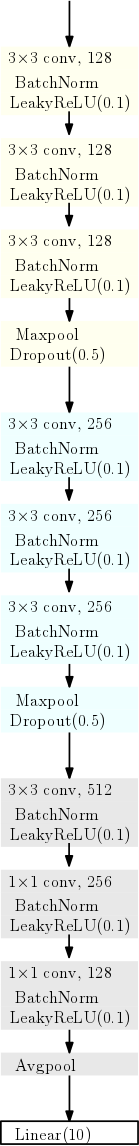
\includegraphics[scale=0.6]{report/figures/net.png}
    \caption{The network architecture: three blocks, each consisting of three convolution layers, and a linear layer for classification.}
    \label{fig:net}
\end{figure}

\onecolumn

\begin{table}
    \centering
    \begin{tabular}{|r|c|c|c|c|}
    \hline
                    & \multicolumn{4}{|c|}{StepLR (step size=30)}            \\ \hline
    momentum        & \multicolumn{2}{|c|}{0.9} & \multicolumn{2}{|c|}{0.95}\\ \hline
    weight decay    & $1e^{-3}$ & $1e^{-4}$     & $1e^{-3}$ & $1e^{-4}$     \\ \hline
    accuracy        & $49.73\%$ & $49.80\%$     & $49.01\%$ & $ 48.85\%$    \\ \hline
    \end{tabular}
    
    \bigskip
    \begin{tabular}{|r|c|c|c|c|}
    \hline
                    & \multicolumn{4}{|c|}{CosineAnnealingLR ($t_{max}$=100)}            \\ \hline
    momentum        & \multicolumn{2}{|c|}{0.9} & \multicolumn{2}{|c|}{0.95}\\ \hline
    weight decay    & $1e^{-3}$ & $1e^{-4}$     & $1e^{-3}$ & $1e^{-4}$     \\ \hline
    accuracy        & $51.16\%$ & $50.01\%$     & $51.62\%$ & $50.48\%$    \\ \hline
    \end{tabular}
        
    \bigskip
    \begin{tabular}{|r|c|c|c|c|}
    \hline
                    & \multicolumn{4}{|c|}{CosineAnnealingWarmRestarts ($t_0$=10)}            \\ \hline
    momentum        & \multicolumn{2}{|c|}{0.9} & \multicolumn{2}{|c|}{0.95}\\ \hline
    weight decay    & $1e^{-3}$ & $1e^{-4}$     & $1e^{-3}$ & $1e^{-4}$     \\ \hline
    accuracy        & $52.59\%$ & $51.20\%$     & $50.90\%$ & $50.41\%$    \\ \hline
%  lr=0.1           & 50.34\%   %    
    \end{tabular}
    \caption{Evaluation results on our changes to increase the baseline accuracy of our network while training for 100 epochs at learning rate of 0.01. The first table shows accuracy when using the \texttt{StepLR} learning rate scheduler with varying momentum and weight decay, the second one the \texttt{CosineAnnealingLR}, and the third one the \texttt{CosineAnnealingWarmRestarts}. Entries show the average accuracy over five runs.}
    \label{tab:baseexp}
\end{table}{}
\section{Experiments}
\label{sec:experiments}

We apply manifold mixup regularization on our best baseline model that is summarized in table~\ref{tab:baseline}.
We experimented with different $\alpha$ values and all possible combinations of eligible layers $\mathcal{S}$. 
The first layers of the three blocks of our network architecture are the set of all eligible layers.
Furthermore, $\mathcal{S} = \{0\}$ means input mixup as in~\cite{zhang17}.
If $|\mathcal{S}| > 1$ then a layer $k \in \mathcal{S}$ is chosen at random before a minibatch is processed during training as done in~\cite{verma19}.

\begin{table}[H]
    \centering
    \begin{tabular}{ccccccc}
        \toprule
        epochs & optimizer & lr & momentum & weight decay & $t_0$ & accuracy \\
        \midrule
        $400$ & SGD & $0.1$ & $0.9$ & $1e^{-3}$ & $10$ & $56.07\%$ \\
        \bottomrule
    \end{tabular}
    \caption{Our final baseline model}
    \label{tab:baseline}
\end{table}

Table~\ref{tab:experiments} lists our evaluations with a multitude of different $\alpha$-values and eligible layers $\mathcal{S}$. As described in section~\ref{sec:introduction}, $\alpha$ controls the strength of the mixup applied to one randomly selected layer from the set of eligible layers $\mathcal{S}$.

Our results show that applying manifold mixup regularization has a positive effect regardless of where and how strongly applied compared to our baseline. Allowing mixup at the last layer only yields the least improvements. On the other hand, in most experiments allowing mixup at both, the input layer and the last layer, outperformed all other combinations of eligible layers with an increase in accuracy of $2.74\%$ to $5.66\%$ compared to our baseline model.

When looking at the influence of the hyperparameter $\alpha$, the overall best performance  can be observed at $\alpha=4.0$, with an average accuracy of $60,17\%$, and $\alpha=2.0$ with $60.12\%$. Considering that $\alpha$ controls the mixup strength based on the beta-distribution, our findings suggest that a strong mixup, i.e., a mixup factor $\lambda$ with a high probability of being close to $0.5$, has indeed a positive influence on the results.
% interactive beta distribution thingy: https://demonstrations.wolfram.com/BetaDistribution/

The overall best test set accuracy was achieved with the configuration of $\mathcal{S}=\{0,2\}$ and $\alpha=4.0$, with an increase in accuracy of $5.66\%$ compared to the baseline, and an improvement of $0.97\%$ compared to our best accuracy using only input mixup ($\mathcal{S}=\{0\}$).



\begin{table}[H]
    \centering
    \begin{tabular}{c|ccccccc}
        \toprule
        \multirow{2}{*}{$\mathcal{S}$} & \multicolumn{7}{|c}{$\alpha$} \\
        & 0.2 & 0.5 & 1.0 & 1.5 & 2.0 & 4.0 & 5.0\\ 
        \midrule
        $\{ 0 \}$       & $58.66$ & $59.06$ & $60.36$ & $60.76$ & $60.41$ & $59.91$ & $60.33$ \\
        $\{ 1 \}$       & $58.07$ & $58.87$ & $59.09$ & $58.86$ & $59.50$ & $59.01$ & $58.43$\\
        $\{ 2 \}$       & $57.51$ & $57.38$ & $57.46$ & $57.80$ & $57.86$ & $58.36$ & $57.79$\\
        $\{ 0, 1 \}$    & $58.45$ & $59.64$ & $60.08$ & $\bm{61.09}$ & $61.20$ & $60.96$ & $61.21$ \\
        $\{ 0, 2 \}$    & $\bm{58.80}$ & $\bm{59.76}$ & $60.67$ & $60.16$ & $\bm{61.33}$ & $\bm{61.73}$ & $\bm{61.61}$\\
        $\{ 1, 2 \}$    & $57.73$ & $58.56$ & $59.37$ & $59.32$ & $59.69$ & $59.79$ & $59.37$\\
        $\{ 0, 1, 2 \}$ & $58.29$ & $59.25$ & $\bm{61.13}$ & $60.76$ & $60.87$ & $61.44$ & $61.05$\\
        
        \bottomrule
    \end{tabular}
    \caption{Test set accuracies using manifold mixup regularization with different mixing coefficients $\alpha$.}
    \label{tab:experiments}
\end{table}

% ~~~~~~~~~~~~~~~~~~~~~~~~~~~~~~~~ %
% ~~~~~~~~~ NEW Results ~~~~~~~~~~ %
% ~~~~~~~~~~~~~~~~~~~~~~~~~~~~~~~~ %

% alpha=0.2
    % Mixup Config: [True, False, False]
    % Accuracy after 5 iterations: 58.66%
    % Mixup Config: [False, True, False]
    % Accuracy after 5 iterations: 58.07%
    % Mixup Config: [False, False, True]
    % Accuracy after 5 iterations: 57.51%
    % Mixup Config: [True, True, False]
    % Accuracy after 5 iterations: 58.45%
    % Mixup Config: [True, False, True]
    % Accuracy after 5 iterations: 58.80%
    % Mixup Config: [False, True, True]
    % Accuracy after 5 iterations: 57.73%
    % Mixup Config: [True, True, True]
    % Accuracy after 5 iterations: 58.29%

% alpha=0.5
    % Mixup Config: [True, False, False]
    % Accuracy after 5 iterations: 59.06%
    % Mixup Config: [False, True, False]
    % Accuracy after 5 iterations: 58.87%
    % Mixup Config: [False, False, True]
    % Accuracy after 5 iterations: 57.38%
    % Mixup Config: [True, True, False]
    % Accuracy after 5 iterations: 59.64%
    % Mixup Config: [True, False, True]
    % Accuracy after 5 iterations: 59.76%
    % Mixup Config: [False, True, True]
    % Accuracy after 5 iterations: 58.56%
    % Mixup Config: [True, True, True]
    % Accuracy after 5 iterations: 59.25%
    
% alpha=1.0
    % Mixup Config: [True, False, False]
    % Accuracy after 5 iterations: 60.36%
    % Mixup Config: [False, True, False]
    % Accuracy after 5 iterations: 59.09%
    % Mixup Config: [False, False, True]
    % Accuracy after 5 iterations: 57.46%
    % Mixup Config: [True, True, False]
    % Accuracy after 5 iterations: 60.08%
    % Mixup Config: [True, False, True]
    % Accuracy after 5 iterations: 60.67%
    % Mixup Config: [False, True, True]
    % Accuracy after 5 iterations: 59.37%
    % Mixup Config: [True, True, True]
    % Accuracy after 5 iterations: 61.13%


% alpha=1.5
    % Mixup Config: [True, False, False]
    % Accuracy after 5 iterations: 60.76%
    % Mixup Config: [False, True, False]
    % Accuracy after 5 iterations: 58.86%
    % Mixup Config: [False, False, True]
    % Accuracy after 5 iterations: 57.80%
    % Mixup Config: [True, True, False]
    % Accuracy after 5 iterations: 61.09%
    % Mixup Config: [True, False, True]
    % Accuracy after 5 iterations: 60.16%
    % Mixup Config: [False, True, True]
    % Accuracy after 5 iterations: 59.32%
    % Mixup Config: [True, True, True]
    % Accuracy after 5 iterations: 60.76%

% alpha=2.0
    % Mixup Config: [True, False, False]
    % Accuracy after 5 iterations: 60.41%
    % Mixup Config: [False, True, False]
    % Accuracy after 5 iterations: 59.50%
    % Mixup Config: [False, False, True]
    % Accuracy after 5 iterations: 57.86%
    % Mixup Config: [True, True, False]
    % Accuracy after 5 iterations: 61.20%
    % Mixup Config: [True, False, True]
    % Accuracy after 5 iterations: 61.33%
    % Mixup Config: [False, True, True]
    % Accuracy after 5 iterations: 59.69%
    % Mixup Config: [True, True, True]
    % Accuracy after 5 iterations: 60.87%
    
% alpha=4.0
%     Mixup Config: [True, False, False]
%     Accuracy after 5 iterations: 59.91%
%     Mixup Config: [False, True, False]
%     Accuracy after 5 iterations: 59.01%
%     Mixup Config: [False, False, True]
%     Accuracy after 5 iterations: 58.36%
%     Mixup Config: [True, True, False]
%     Accuracy after 5 iterations: 60.96%
%     Mixup Config: [True, False, True]
%     Accuracy after 5 iterations: 61.73%
\section{Summary}
\label{sec:summary}

\dots

\bibliography{references}{}
\bibliographystyle{apalike}

\end{document}